\section*{Problems}
%
\begin{enumerate}[itemsep=6pt]
%  \question A ball is attached to a string and whirled in a vertical circle.
%  The tension in the string will be the least
%  \begin{choices}
%    \choice at the bottom of the circle
%    \choice at the top of the circle
%    \choice as the ball is moving towards the top of the circle
%    \choice as the ball is moving towards the bottom of the circle
%    \choice Trick question! Tension will be the same at all points in the
%    circle.
%  \end{choices}
%
%  \question A girl stands on a rotating merry-go-round without holding on to a
%  rail. The force that keeps her moving in a circle is the
%  \begin{choices}
%    \choice frictional force on the girl directed away from the centre of
%    the merry-go-round
%    \choice frictional force on the girl directed towards the centre of the
%    merry-go-round
%    \choice normal force on the girl directed away from the centre of the
%    merry-go-round
%    \choice normal force on the girl directed towards the centre of the
%    merry-go-round
%    \choice weight of the girl
%  \end{choices}
%  
%  \item A bicycle wheel has a radius of 0.5 m. When it spins, it completes
%  one full turn in 1.6 s. A pebble wedged in the tread has a mass of 10 g. What
%  is the centripetal force on the pebble?
%  \begin{choices}
%    \choice\SI{.01}\newton
%    \choice\SI{.08}\newton
%    \choice\SI{.1}\newton
%    \choice\SI{.8}\newton
%    \choice\SI1\newton
%  \end{choices}
%  
%  \item A tetherball swings in a horizontal circle. If the radius of the
%  swing is tripled but the tangential speed remains the same, by what factor
%  does the centripetal force change?
%  \begin{choices}
%    \choice Nine times greater
%    \choice Three times greater
%    \choice Remains the same
%    \choice One-third as much
%    \choice One-ninth as much
%  \end{choices}
%  
%  \item A car of mass $m$ drives on a flat circular track of radius $R$. To
%  maintain a constant speed $\varv$ on the track, the coefficient of friction
%  $\mu$ between the tires and the road must be
%  \begin{choices}
%    \choice $mg$
%    \choice $mg+\dfrac{m\varv^2}R$
%    \choice $mg-\dfrac{m\varv^2}R$
%    \choice $\dfrac{\varv^2}{gR}$
%    \choice $\sqrt{\dfrac{\varv^2}{gR}}$
%  \end{choices}
%  \newpage
%  
%  \item A car travels on a circular track that is banked at an angle
%  $\theta$ from the horizontal, as shown in the diagram below. Which of the
%  following diagrams best shows the forces acting on the car as it moves on the
%  banked track?
%  \begin{center}
%    \vspace{-.1in}
%    \pic{.18}{../graphics/banked-turn-acceleration}
%  \end{center}
%
%  \vspace{-.15in}
%  A.\begin{tikzpicture}
%    \fill circle (.08);
%    \draw[vectors] (0,0)--(0,1) node[above]{$\vec N$};
%    \draw[vectors] (0,0)--(0,-1) node[below]{$m\vec g$};
%    \draw[vectors,rotate=60] (0,0)--(0,1) node[left]{$\vec F_s$};
%  \end{tikzpicture}
%  \hspace{.2in}
%  B.\begin{tikzpicture}
%    \fill circle (.08);
%    \draw[vectors,rotate=-30] (0,0)--(0,1) node[above]{$\vec N$};
%    \draw[vectors,rotate=-30] (0,0)--(0,-1) node[below]{$m\vec g$};
%    \draw[vectors,rotate=60] (0,0)--(0,-1) node[right]{$\vec F_s$};
%  \end{tikzpicture}
%  \hspace{.2in}
%  C.\begin{tikzpicture}
%    \fill circle (.08);
%    \draw[vectors,rotate=-30] (0,0)--(0,1) node[above]{$\vec N$};
%    \draw[vectors] (0,0)--(0,-1) node[below]{$m\vec g$};
%    \draw[vectors,rotate=60] (0,0)--(0,-1) node[right]{$\vec F_s$};
%  \end{tikzpicture}
%  \hspace{.2in}
%  D.\begin{tikzpicture}
%    \fill circle (.08);
%    \draw[vectors] (0,0)--(0,1) node[above]{$\vec N$};
%    \draw[vectors] (0,0)--(0,-1) node[below]{$m\vec g$};
%    \draw[vectors,rotate=60] (0,0)--(0,-1) node[right]{$\vec F_s$};
%  \end{tikzpicture}
%  \hspace{.2in}
%  E. \begin{tikzpicture}
%    \fill circle (.08);
%    \draw[vectors,rotate=120] (0,0)--(0,1) node[left]{$\vec N$};
%    \draw[vectors] (0,0)--(0,-1) node[below]{$m\vec g$};
%    \draw[vectors,rotate=60] (0,0)--(0,-1) node[right]{$\vec F_s$};
%  \end{tikzpicture}
%  
%  \item In the previous question, which of the following statements is true
%  of the forces acting on the car while on the circular track?
%  \begin{choices}
%    \choice The normal force the track exerts on the car provides the
%    centripetal force.
%    \choice The weight of the car provides the centripetal force.
%    \choice The frictional force the track exerts on the car provides the
%    centripetal force.
%    \choice The centripetal force is provided by a combination of the normal
%    force and frictional force.
%    \choice There is no centripetal force in this case.
%  \end{choices}
%  
%  \item When drawing free-body diagrams, does the label ``centripetal
%  force'' get used? Explain.
%  \vspace{\stretch1}
  
\item A car exits a highway on a ramp that is banked at \ang{15} with a radius
  of curvature of \SI{65}\metre. If the ramp is extremely icy and the driver
  cannot depend on any friction to help make the turn, what is the safe speed
  that the driver can travel so that the car will not skid off the ramp? 
  
\item A highway curve with a radius of curvature of \SI{155}{\metre} must
  accommodate cars travelling at \SI{50}{\kilo\metre\per\hour} without
  friction. At what angle should the curve be banked? (Be careful with unit
  conversion.)

\item A pilot of mass \SI{68.5}{\kilo\gram} in a jet aircraft makes a complete
  vertical circle in mid-air. The vertical circle has a radius of
  \SI{1.70}{\kilo\metre}. The speed of the jet is \SI{215}{\metre\per\second}.
  Draw a free-body diagram of the forces acting on the pilot, determine the
  force of the seat on the pilot at
  \begin{enumerate}[itemsep=3pt]
  \item the bottom of the loop and
  \item the top of the loop
  \end{enumerate}
  (Note that at the top of the loop, the aircraft is upside down.)
 
\item A boy is twirling a \SI{555}{\gram} ball on a \SI{65.0}{\centi\metre}
  string in a \emph{horizontal} circle. The string will break if the tension
  reaches \SI{15.0}\newton.
  \begin{enumerate}[itemsep=3pt]
  \item On the dot below, draw and label all the forces (not components) that
    act on the ball. Forces should be drawn as arrows originating at, and
    pointing away from, the dot. (Hint: Tension force $F_T$ does \emph{not}
    point towards the centre of the circular motion. Since the ball moves in a
    horizontal path, the vertical component of the net force must be zero.
    The horizontal component is the centripetal force. This is similar to the
    in-class example of an airplane turning.)
%      \begin{center}
%        \vspace{1in}
%      {\tikz\fill circle (.15);}
%      \vspace{1in}
%    \end{center}        

  \item Find the centripetal force when tension is at maximum? (Hint: It may be
    easier to solve the problem algebraically first, before substituting
    numerical values. The centripetal force is \emph{not} \SI{15.0}\newton.)
    
  \item What is the maximum speed at which the ball can move without breaking
    the string? (Hint: Once the centripetal force is found, you can find the
    centripetal acceleration. The tricky part of this question is to find the
    radius of the motion. It is  \emph{not} \SI{65.0}{\centi\metre}.)
  \end{enumerate}

\begin{center}
  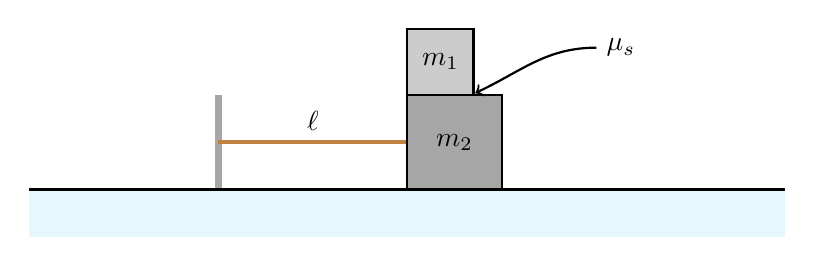
\begin{tikzpicture}[scale=1.2]
    \fill[cyan!10] rectangle (8,-.5);
    \draw[gray!70,line width=2.5] (2,0)--(2,1);
    \draw[brown,ultra thick] (2,.5)--(4,.5) node[midway,above,black]{$\ell$};
    \draw[thick,fill=gray!70] (4,0) rectangle +(1,1) node[midway]{$m_2$};
    \draw[thick,fill=gray!40] (4,1) rectangle +(.7,.7) node[midway]{$m_1$};
    \draw[very thick] (0,0)--(8,0);
    \draw[<-,thick] (4.72,1.02) to[out=25,in=180](6,1.5) node[right]{$\mu_s$};
  \end{tikzpicture}
\end{center}
\item Mass $m_1$ (\SI{2.0}{\kilo\gram}) sits on top of mass $m_2$
  (\SI{5.0}{\kilo\gram}), which rests on a frictionless table, as shown above.
  The coefficient of static friction between the two masses is $\mu_s=0.30$. A
  string of length $\ell=\SI{5.0}\metre$ is tied to $m_2$, and both masses
  are swung around without slipping in a horizontal circle.
  \begin{enumerate}[itemsep=3pt]
  \item On the dots below, draw and label all the forces (not components) that
    act on the masses. Forces should be drawn as arrows originating at, and
    pointing away from, the dots that represent the masses. (Hint: There are
    normal force at all contacts between the masses and the table.)
    %\begin{center}
    %  \begin{tikzpicture}
    %    \fill circle (.1) node[left]{$m_1$};
    %    \fill (7,0) circle (.1) node[left]{$m_2$};
    %  \end{tikzpicture}
    %\end{center}

  \item Calculate the maximum centripetal acceleration of the masses. (Hint:
    This is a multi-body problem like the stacked-body example studied in Class
    2, except in this case, we are solving for the maximum \emph{centripetal}
    acceleration. The top mass $m_1$ accelerates because of static friction.)
    
  \item Calculate the maximum speed of the masses. (Once you have the
    centripetal acceleration, this should be very simple.)
    
  \item Calculate the tension in the string when the masses are moving at
    maximum speed.
  \end{enumerate}

  \begin{center}
    \pic{.5}{circularMotion/graphics/twoblocks}
  \end{center}
  
\item A block of mass $m_1$ is attached to a cord of length $L_1$, which
  is fixed at one end. The mass moves in a horizontal circle supported by a
  frictionless table. A second block of mass $m_2$ is attached to the first by
  a cord of length $L_2$ and also moves in a circle, as shown in the diagram.
  If the period of the motion is $T$:
  \begin{enumerate}[itemsep=3pt]
  \item On the dots below, draw and label all the forces (not components) that
    act on the blocks. Forces should be drawn as arrows originating at, and
    pointing away from, the dots that represent the blocks.
    %\begin{center}
    %  \vspace{1in}
    %  \begin{tikzpicture}
    %    \fill circle (.1) node[left]{$m_1$};
    %    \fill (7,0) circle (.1) node[left]{$m_2$};
    %  \end{tikzpicture}
    %  \vspace{1in}
    %\end{center}    
  \item Find the tension in each cord.
  \end{enumerate}
\end{enumerate}

